% Background Section

\section{Background}

\begin{frame}{Related Work}
\begin{columns}
\begin{column}{0.5\textwidth}
\textbf{Legal NLP Research:}
\begin{itemize}
    \item Contract analysis (Katz et al., 2020)
    \item Legal document classification
    \item Information extraction from legal texts
\end{itemize}

\vspace{0.5cm}
\textbf{Explainable AI Methods:}
\begin{itemize}
    \item Model-agnostic approaches
    \item Attention mechanisms
    \item Feature attribution methods
\end{itemize}
\end{column}
\begin{column}{0.5\textwidth}
\textbf{Gaps in Current Research:}
\begin{itemize}
    \item Limited comparison of XAI methods
    \item Lack of domain-specific evaluation
    \item Insufficient user studies in legal domain
\end{itemize}

\vspace{0.5cm}
\textbf{Our Contribution:}
\begin{itemize}
    \item \highlight{Multi-method} explainability comparison
    \item \highlight{Legal-specific} evaluation metrics
    \item \highlight{Comprehensive} visualization toolkit
\end{itemize}
\end{column}
\end{columns}
\end{frame}

\begin{frame}{Technical Background}
\begin{block}{BERT (Bidirectional Encoder Representations from Transformers)}
\begin{itemize}
    \item Pre-trained on large text corpus
    \item Bidirectional context understanding
    \item Fine-tunable for specific tasks
\end{itemize}
\end{block}

\begin{block}{Explainability Methods}
\begin{description}
    \item[SHAP] Game-theoretic approach to feature attribution
    \item[LIME] Local surrogate models for instance-specific explanations
    \item[Attention] Built-in transformer attention weights
\end{description}
\end{block}
\end{frame}

\begin{frame}{Dataset Overview}
\begin{columns}
\begin{column}{0.6\textwidth}
\textbf{Data Sources:}
\begin{itemize}
    \item Legal contract databases
    \item Public domain agreements
    \item Synthetic legal text generation
\end{itemize}

\vspace{0.5cm}
\textbf{Preprocessing Steps:}
\begin{enumerate}
    \item Text cleaning and normalization
    \item Clause boundary detection
    \item Label annotation and verification
    \item Train/validation/test split
\end{enumerate}
\end{column}
\begin{column}{0.4\textwidth}
\begin{center}
% Include data flow pipeline figure  
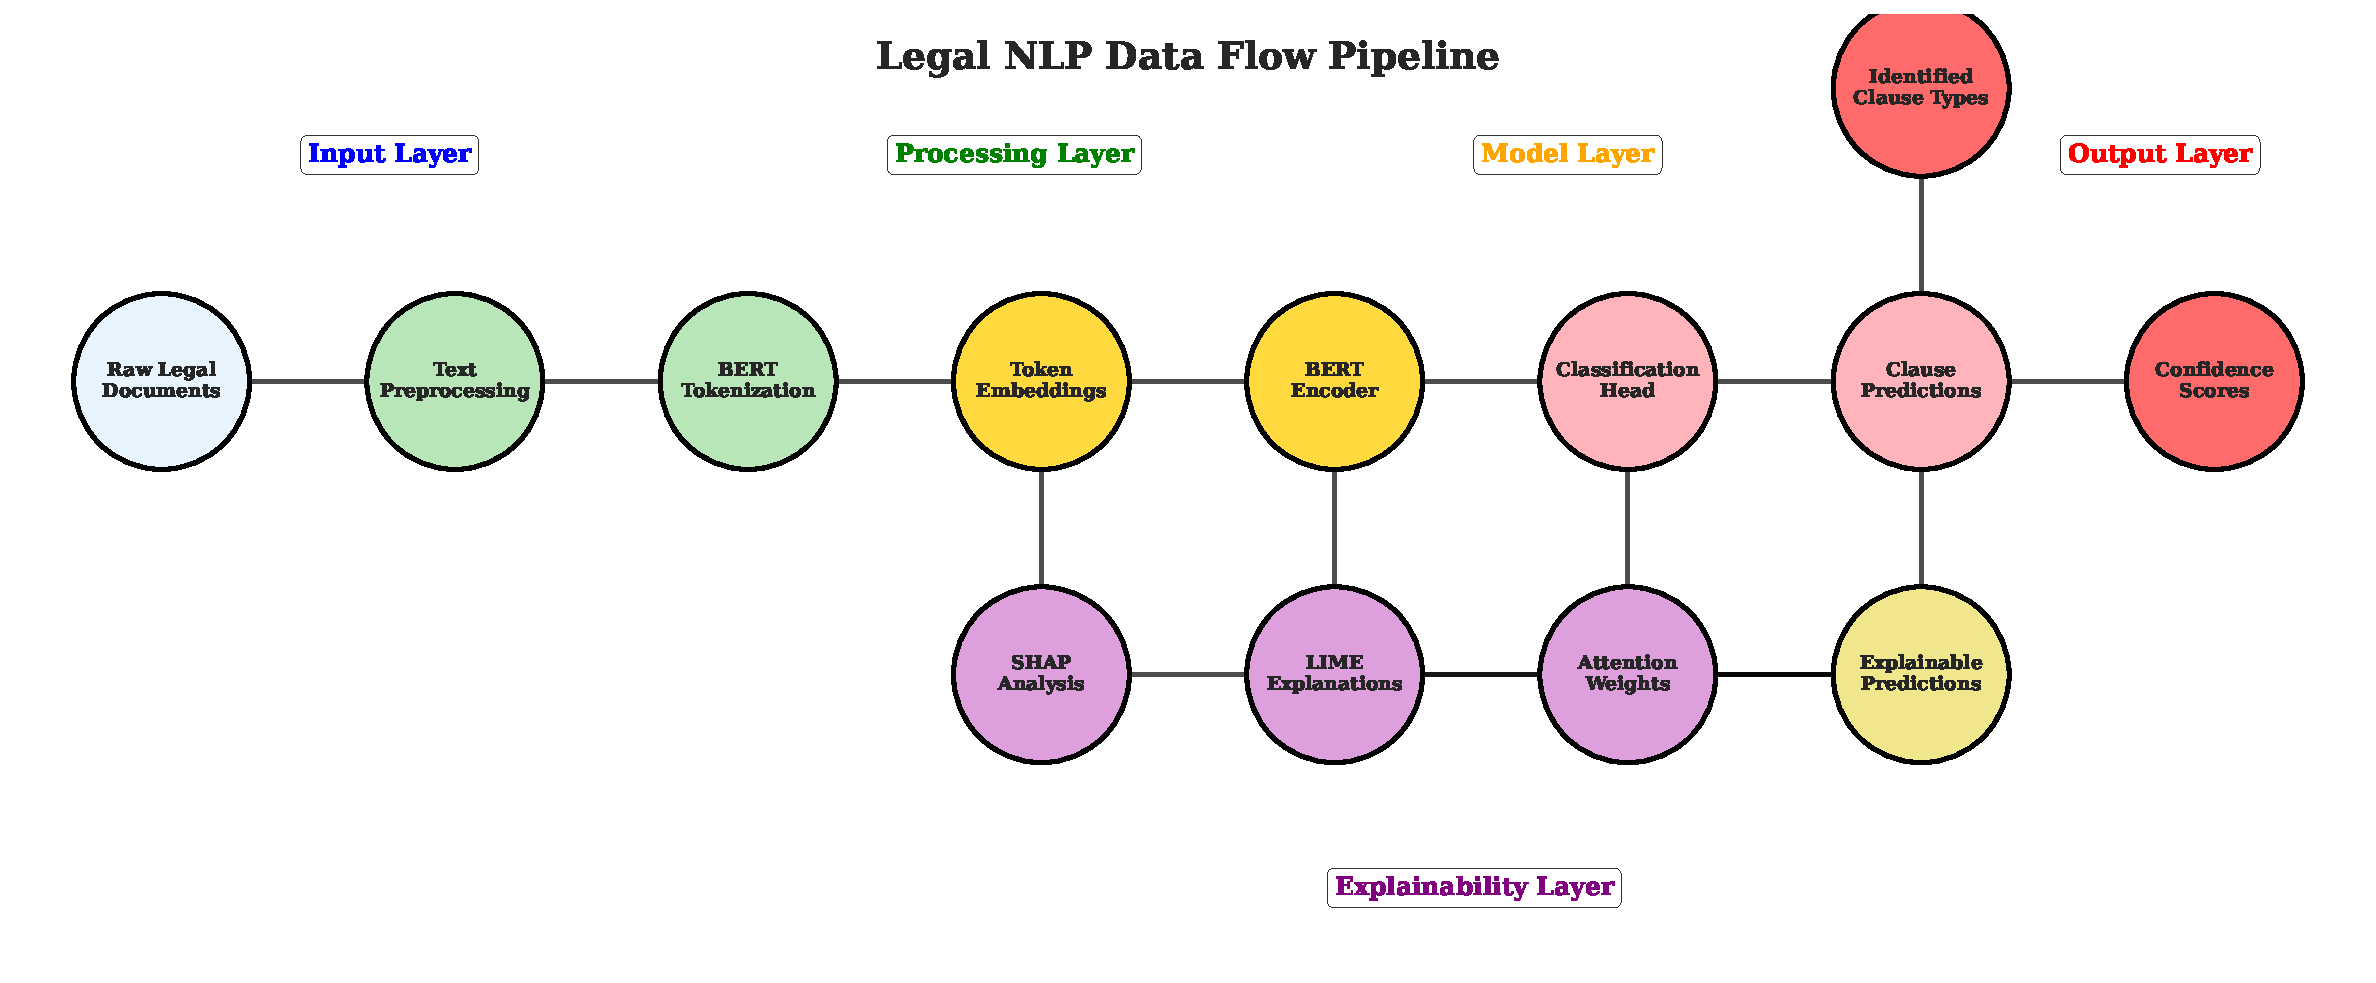
\includegraphics[width=\textwidth]{\figpath/data_flow_pipeline.pdf}
\end{center}
\end{column}
\end{columns}
\end{frame}
